\iffalse
\chapter{Implementarea aplicației}
\label{cap:cap3}

(10–15 pagini)

\begin{itemize}
    \item Descrierea generală a implementării;
    \item Probleme speciale/dificultăți întâmpinate și modalități de rezolvare;
    \item Idei originale, soluții noi;
    \item Se prezintă pe scurt funcționarea sistemului (câteva capturi de ecran în punctele esențiale); nu se insistă deosebit deoarece există prezentare practică
    \item Comunicarea cu alte sisteme și salvarea/stocarea informațiilor;
    \item Interfața cu utilizatorul; 
    \item Se realizează calibrarea hardware și eventual software și se dau detalii despre maniera în care a fost efectuată. 
\end{itemize}

Dacă în Capitolul \ref{cap:cap2} este descrisă arhitectura aplicației la nivel conceptual (cu scheme logice, diagrame UML, structuri de clase, diagrame ER etc.), Capitolul \ref{cap:cap2} descrie implementarea soluției propuse. Această descriere trebuie să urmeze modulele prezentate în capitolul anterior, cu o eventuală referire a acestora. Se pot introduce fragmente semnificative de cod specifice fiecărui modul în parte.

În acest capitol se descrie implementarea practică a proiectului. În mod uzual, puteți insera cod de dimensiuni mici, care este relevant și care se impune a fi comentat în detaliu. Astfel, Listing-ul \ref{code:c_mpi} prezintă un supergreu pas de inițializare a unui program MPI pentru a obține cinstit punctul din oficiu, în care se poate face referire la linia \ref{line:if} pentru a descrie ce face \verb|if|-u' di acolo.

\begin{code}
    \begin{minted}{c}
        #include <stdio.h>
        #include "mpi.h"
        
        int main( int argc, char **argv ) {
        	char message[20];
        	int myrank;	
        		
        	MPI_Status status;
        
        	MPI_Init( &argc, &argv );
        	MPI_Comm_rank( MPI_COMM_WORLD, &myrank );
        	
        	if (myrank == 0) { /* codul pentru procesul 0 */|\label{line:if}|
        		strcpy(message,"Hello");
        		MPI_Send(message, strlen(message), MPI_CHAR, 
        			1, 99, MPI_COMM_WORLD);
        	} else { /* codul pentru procesul 1 */
        		MPI_Recv(message, 20, MPI_CHAR, 
        			0, 99, MPI_COMM_WORLD, &status);
        		printf("received :%s:\n", message);
        	}
        	
        	MPI_Finalize();
        	return 0;
        }
    \end{minted}
    \caption{Supercod MPI în C} 
    \label{code:c_mpi}
\end{code}

Codul complet relevant se va include în anexe (vezi Anexele \ref{anexa6:listing_python}, \ref{anexa7:listing_kotlin} și \ref{anexa8:listing_xml}). De exemplu, Listing-ul \ref{code:xml_pom} (Anexa \ref{anexa8:listing_xml}) prezintă fișierul de configurare \textit{maven} pentru un serviciu SOAP minimal.

\textcolor{gray}{\lipsum}

\textcolor{gray}{\lipsum}
\fi

\chapter{Implementarea aplicației}
\label{cap:cap3}

\section{Implementarea PRNG-urilor}

Problema principală cu implementarea unui PRNG în limbajul Python este faptul că Python folosește implicit numere întregi cu precizie arbitrară (întregii pot să aibe orice dimensiune). Astfel, cum majoritatea algoritmilor de generare de numere aleatorii se bazează pe overflow / underflow intenționat, trebuie realizat o operație în plus de modulo 2 la puterea preciziei dorite (în cazul meu, 32).

Ca orice generator de numere pseudoaletorii, cele două generatoare implementate de mine (LCG și KISS) se bazează pe actualizarea unei stări globale pentru calculul următorii valori. În cazul meu, voi folosi paradigma OOP pentru a stoca această valoare.

Valorile pentru seed-uri sunt luate din recomandările lui George Marsaglia în \cite{misc:usenet:GeorgeMarsaglia}.

În următorul listing de cod voi prezenta clasa PRNG utilizată în cea de-a doua aplicație, cea cu interfața utilizator.

\begin{code}
\begin{minted}{python}
class PRNG:
    def __init__(self):
        self.LCG_rand = 6969
        self.LCG_a = 1664525
        self.LCG_c = 1013904223
        self.m = 2 ** 32
        self.jsr = 123456789
        self.jcong = 380116160
        self.z = 362436069
        self.w = 521288629
    def run_LCG(self, shots):
        numbers = []
        for i in range(shots):
            self.LCG_rand =  (self.LCG_a * self.LCG_rand + self.LCG_c) \
            % self.m
            numbers.append(self.LCG_rand)
        maxim = max(numbers)
        numbers = [round((i / maxim)*255) for i in numbers]
        return numbers
    def run_KISS(self, shots):
        numbers = []
        for i in range(shots):
            self.jsr = (self.jsr ^ ((self.jsr << 17) % self.m)) % self.m
            self.jsr = (self.jsr ^ ((self.jsr >> 13 ) % self.m)) % self.m
            self.jsr = (self.jsr ^ ((self.jsr << 5) % self.m)) % self.m
            self.jcong = ((69069 * self.jcong) % self.m + 1234567) % self.m
            self.z = ((36969 * (self.z & 65535)) % 2 ** 16 + (self.z >> 16))\
            % 2 ** 16
            self.w = ((18000 * (self.w & 65535)) % 2 ** 16 + (self.w >> 16))\
            % 2 ** 16
            mwc = ((self.z << 16) + self.w) % self.m
            numbers.append(mwc)
        maxim = max(numbers)
        numbers = [round((i / maxim)*255) for i in numbers]
        return numbers
\end{minted}
\end{code}

După cum se poate vedea, felul în care am implementat aceste generatoare returnează numere numai între 0 și 255 (fără normalizare pe intervalul [0, 1], așa cum recomandă și George Marsaglia). Acest lucru este din cauză că am vrut să am consecvență cu generatoarele de numere aleatorii cuantice, care sunt limitate la 8 qubiți și pot astfel să genereze numere doar pe intervalul [0, 255]. Totuși, acest lucru a dus la apariția unor probleme destul de mari cu unele teste statistice (testele din suita de teste Diehard și Dieharder recomandate de Marsaglia) datorită lipsei de implementare a acestora pe sisteme cu întregi pe mai puțin de 32 de biți. 

De asemenea, din cauza împărțirilor ca numere reale și a rotunjirii, numerele generate prezintă uneori "creste" cu o perioadă destul de mică, cum voi arăta în capitolul următor.

\section{Implementarea QRNG-urilor}

Înainte de a prezenta implementarea programatică a circuitelor cuantice utilizate (figuri la anexe), voi prezenta mai întâi o funcție ajutătoare: funcția de concatenare 8 câte 8 biți. Acest lucru este posibil doar pentru distribuțiile uniforme deoarele concatenarea a 8 biți cu probabilitate egală pentru cele două valori, 0 și 1, rezultă într-o distribuție uniformă pe toate cele 256 de valori posibile, facând astfel posibilă executarea generatoarelor pe calculatoare cuantice cu orice număr de qubiți. Același lucru nu este totuși posibil pentru circuitele de generare a numerelor aleatorii pe distribuție normală, totuși, motiv pentru am decis să păstrez limitarea numerelor generate pe intervalul [0, 255]. 

\subsection{Funcția de concatenare câte 8 biți}

\begin{code}
\begin{minted}{python}
    def concatenate_bits(self, memory):
        numbers = []
        temp = ''
        c = 0
        for i in range(len(memory)):
            temp = temp + memory[i]
            c = c + 1
            if c == 8:
                numbers.append(temp)
                temp = ''
                c = 0
        numbers = [int(x, 2) for x in numbers]
        return numbers
\end{minted}
\end{code}

Cum numerele returnate de framework-ul qiskit pentru experimentele cu circuite cuantice sunt string-uri, construiesc numărul de 8 biți luând câte 8 simboluri odată din memoria circuitului (cu un singur qubit) și apoi interpretez string-ul rezultat ca un număr pe 8 biți în baza 2.

\subsection{Implementarea (în cod) a generatoarelor de numere aleatorii cuantice}

Cum circuitele utilizate pentru distribuțiile uniforme sunt destul de simple, voi comenta aici pe scurt codul utilizat pentru inițializarea circuitelor.
\begin{code}
\begin{minted}{python}
class QRNG:
    def __init__(self):
        self.sim = Aer.get_backend('aer_simulator')
        self.QC_Hadamard_1bit = QuantumCircuit(1)
        self.QC_Hadamard_1bit.h(0)
        self.QC_RY_1bit = QuantumCircuit(1)
        self.QC_RY_1bit.ry(math.pi/2, 0)
        self.QC_Hadamard_8bit = QuantumCircuit(8)
        self.QC_Hadamard_8bit.h(range(0, 8))
        self.QC_RY_8bit = QuantumCircuit(8)
        self.QC_RY_8bit.ry(math.pi/2, range(0, 8))
        self.QC_Uniform_1bit = UniformDistribution(1)
        self.QC_Uniform_1bit = transpile(self.QC_Uniform_1bit,\
        self.sim, optimization_level=3)
        self.QC_Uniform_8bit = UniformDistribution(8)
        self.QC_Uniform_8bit = transpile(self.QC_Uniform_8bit,\
        self.sim, optimization_level=3)
        
        self.QRNGs = [
            self.QC_Hadamard_1bit, self.QC_Hadamard_8bit, self.QC_RY_1bit,\
            self.QC_RY_8bit, self.QC_Uniform_1bit, self.QC_Uniform_8bit
         ]
        for i in range(len(self.QRNGs)):
            self.QRNGs[i].measure_all()
\end{minted}
\end{code}

Circuitele sunt denumite reprezentativ. Partea interesantă este pasul de transpilare, care pentru calculatoare cuantice adevărate (care au numai anumite basis gates - porți care pot fi de fapt utilizate), iar restul porților trebuiesc descompuse în acestea. Totuși, backend-ul "aer\_simulator" implementează toate aceste porți logice cuantice, iar pasul de transpilare nu face cine știe ce. Este totuși util pentru circuitele care produc numere pe o distribuție normală, pe care le voi discuta mai departe.

Prin urmare, folosesc numai circuite implementate la nivel de poartă logică de mine însumi, urmate de două circuite din biblioteca qiskit.finance, UniformDistribution.

\subsection{Implementarea circuitului pentru distribuție normală, varianta mea}
Funcția care compune un circuit care va returna numere aleatorii pe o distribuțue normală este următoarea:
\begin{code}
\begin{minted}{python}
    def create_normal_circuit(self, size):
        x = np.linspace(-6, 6, num=2**size)
        probabilities = stats.multivariate_normal.pdf(x, 1, 1)
        normalized_probabilities = probabilities / np.sum(probabilities)
        qc_normal = QuantumCircuit(size)
        initial = Initialize(np.sqrt(normalized_probabilities))
        distribution = initial.gates_to_uncompute().inverse()
        qc_normal.compose(distribution, inplace=True)
        return qc_normal
\end{minted}
\end{code}
În acest fel, generez o funcție densitate de probabilitate pornind de la un spațiu liniar cu valori între extreme (parametrul bounds de la circuitul NormalDistribution din biblioteca qiskit.finance) - adică voi lua 256 de valori la spații egale între valorile [-6, 6]. Apoi, calculez radicalii probabilităților individuale din funcția densitate probabilitate (pentru a inițializa șansele ca un qubit să colapseze în starea $\ket{0}$), după care inversez probabilitățile în circuitul compus pentru a obține șansele de colaps în $\ket{1}$. 

Circuitul rezultat este mult prea mare pentru a putea fi afișat prin metode convenționale. O mică parte apare în figura următoare:
\begin{figure}[H]
    \centering
    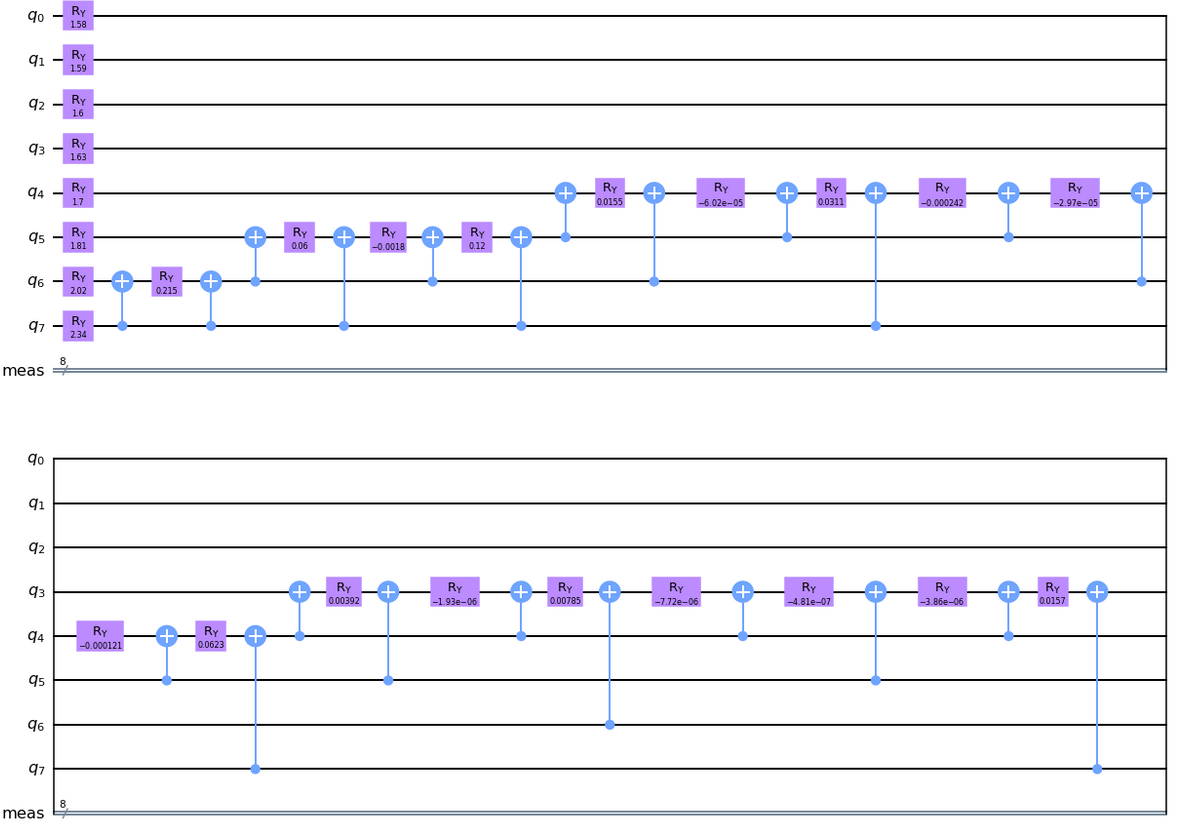
\includegraphics[width=1.0\textwidth]{continut/capitol3/figuri/CircuitNormal.png}
    \label{fig:CircuitNormal}
\end{figure}

\section{Implementarea testelor statistice}

\subsection{Testul Z}
Felul în care am implementat testul Z este un forma two-tailed pentru compararea mediilor a două eșantioane cu varianțe inegale. Astfel, formula pentru calculul parametrului Z în acest caz este
\begin{code}
\begin{minted}{python}
z_calc = (df['counts'].mean() - df2['counts'].mean()) /\
(math.sqrt(df.var()['counts'] / len(df['counts']) + df2.var()['counts'] /\
len(df2['counts'])))
\end{minted}
\end{code}

unde df reprezintă un DataFrame pandas care conține pe o coloană una dintre valorile posibile (un întreg pe intervalul [0, 255]) și pe cealaltă numărul de apariții a acelui număr în totalitatea numerelor generate, iar df2 reprezintă același lucru, dar pentru o distribuție care "se știe" a fi uniformă (în cazul meu, generată cu numpy.random.randint din biblioteca numpy).
\subsection[Testul chi pătrat]{Testul $\chi^2$}
Forma de test chi pătrat implementată de mine este cea propusă în \cite{art:PetrilaMantaUnguranu:IEEESystheory:2014}. Astfel, testul este implementat în felul următor:

\begin{code}
\begin{minted}{python}
    interval = [0, 32]
    sum = 0
    for i in range(0, 8):
        interval[0] = 32 * i
        interval[1] = 32 * i + 32
        count = np.count_nonzero((nums >= interval[0]) & (nums < interval[1]))
        sum += (count - len(nums) / 8) ** 2
    score = ( 8 / (len(nums) * 7) ) * sum
\end{minted}
\end{code}
Unde intervalele se iau 32 câte 32 (mai intâi [0, 32], apoi [32, 64], etc. ) pentru a împărți cele 256 de valori posibile în 8 intervale.

Pentru vizualizarea implementării celorlalte teste statistice, vedeți anexa \ref{anexa3:TesteStatistice}.

\section{Interfața cu utilizatorul}
Aplicația cu interfață cu utilizatorul a fost, cum am menționat în capitolul precedent, implementată cu ajutorul framework-ului PySimpleGUI.Astfel, aceasta arată în felul următor:
\begin{figure}[H]
    \centering
    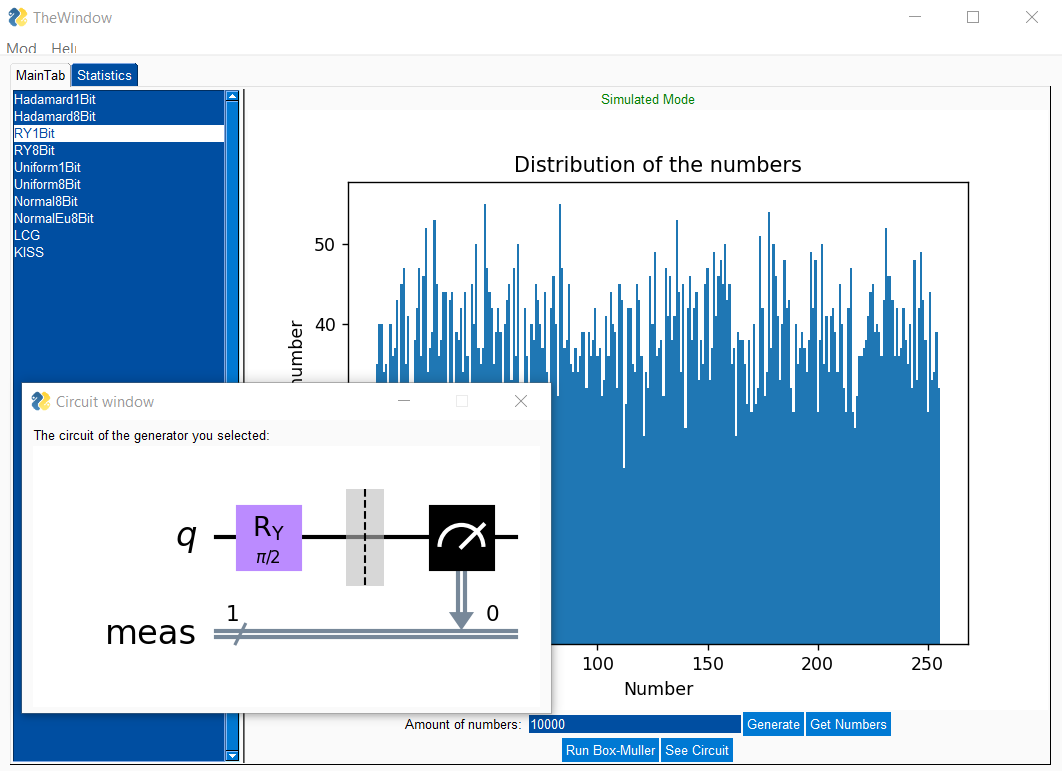
\includegraphics[width=1.0\textwidth]{continut/capitol3/figuri/InterfataCircuit.png}
    \caption{Interfața după execuția unui circuit, cu circuitul afișat}
    \label{fig:InterfataCircuit}
\end{figure}
Figura reprezintă histograma numerelor generate. 

După apăsarea butonului "Get Numbers", apare o fereastră în felul următor:

\begin{figure}[H]
    \centering
    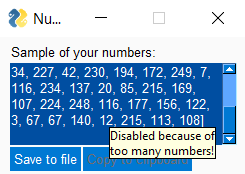
\includegraphics{continut/capitol3/figuri/Numere.png}
    \caption{Fereastra cu numerele generate}
    \label{fig:FereastraNumere}
\end{figure}
Numerele din TextBox reprezintă un eșantion reprezentativ (prima a suta parte din totalul numerelor generate). După apăsarea butoului "Save to file", apare o fereastră specifică sistemului de operare pentru salvarea numerelor în format plain text. Butonul "copy to clipboard" este dezactivat pentru payload-uri de numere mai mari de 4 KB datorită unor limitări în implementare (am dorit a nu folosi unele biblioteci specializate pentru copiat in clipboard, așadar am fost destul de limitat în metode de implementare).

Asupra numerelor generate se execută implicit și testele statistice, împreună cu generarea altor câtorva statistici descriptive. Acestea pot fi vizualizate în tab-ul "Statistics", în felul următor:
\begin{figure}[H]
    \centering
    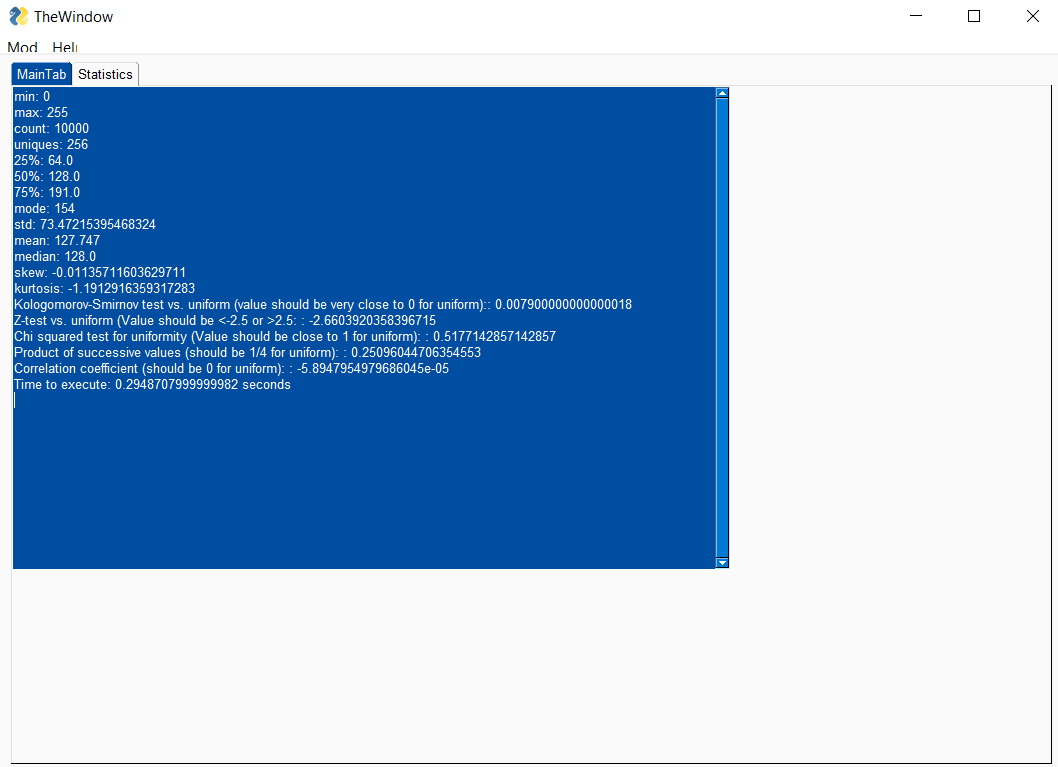
\includegraphics[width=1.0\textwidth]{continut/capitol3/figuri/Statistici.png}
    \caption{Tab-ul cu statisticile}
    \label{fig:StatisticsWindow}
\end{figure}

Semnificațiile sunt explicate în tabelul următor:
\begin{table}[H]
    \centering
    \begin{tabular}{|c|c|}
        \hline
        Statistic & Explanation \\
        \hline  
         min, max & Numerele din extremele distribuției  \\
         count & cantitatea de numere în distribuție  \\
         uniques & cantitatea de numere unice în distribuție \\
         25\%, 50\%, 75\% & quartilele 25, 50 și 75 la sută \\
         mode & modul, adică valoarea care apare cel mai des în distribuție \\
         std & abaterea standard - dispersia valorilor în jurul valorii medii \\
         mean & media aritmetică a valorilor din distribuție \\
         median & mediana (valoarea de mijloc în distribuția sortată) \\
         skew & skewness-ul reprezintă gradul de asimetricitate a distribuției \\
         kurtosis & "măsura de direcționare" reprezintă aglomerarea în jurul mediei \\
         testele statistice & sunt explicate în partea teoretică și în tab\\
        \hline
    \end{tabular}
    \caption{Explicațiile statisticilor din tab-ul "statistics"}
    \label{tab:StatisticsExplainTable}
\end{table}

Pentru implementarea aplicației cu interfață utilizator, vedeți anexa \ref{anexa2:GUIApp}.

\section{Implementarea transformatei Box-Muller}
\begin{code}
\begin{minted}[breaklines, tabsize=1]{python}
def Box_Muller(u1, u2):
    u1 = np.array(u1)
    u2 = np.array(u2)
    u1 = u1 / max(u1)
    u2 = u2 / max(u2)
    z1 = np.sqrt(-2 * np.log(u1, where=u1>0)) * np.cos(2 * math.pi * u2)
    z2 = np.sqrt(-2 * np.log(u1, where=u1>0)) * np.sin(2 * math.pi * u2)
    z1 = np.round_((z1 / max(z1))*255)
    z2 = np.round_((z2 / max(z2))*255)
    z1 = np.nan_to_num(z1)
    z2 = np.nan_to_num(z2)
    return (z1.tolist(), z2.tolist())
\end{minted}
\end{code}
